\documentclass{article}
\usepackage{graphicx} % Required for inserting images
\usepackage{amsmath}
\usepackage{listings}
\usepackage[hidelinks]{hyperref}
\usepackage{float}


\title{Wireless Networks Second Exercise Set Master}
\author{Fotis Bistas}
\date{April 2025}


\begin{document}

\maketitle
\tableofcontents

\section{Introduction and Topology}
\begin{figure}[H]
    \centering
    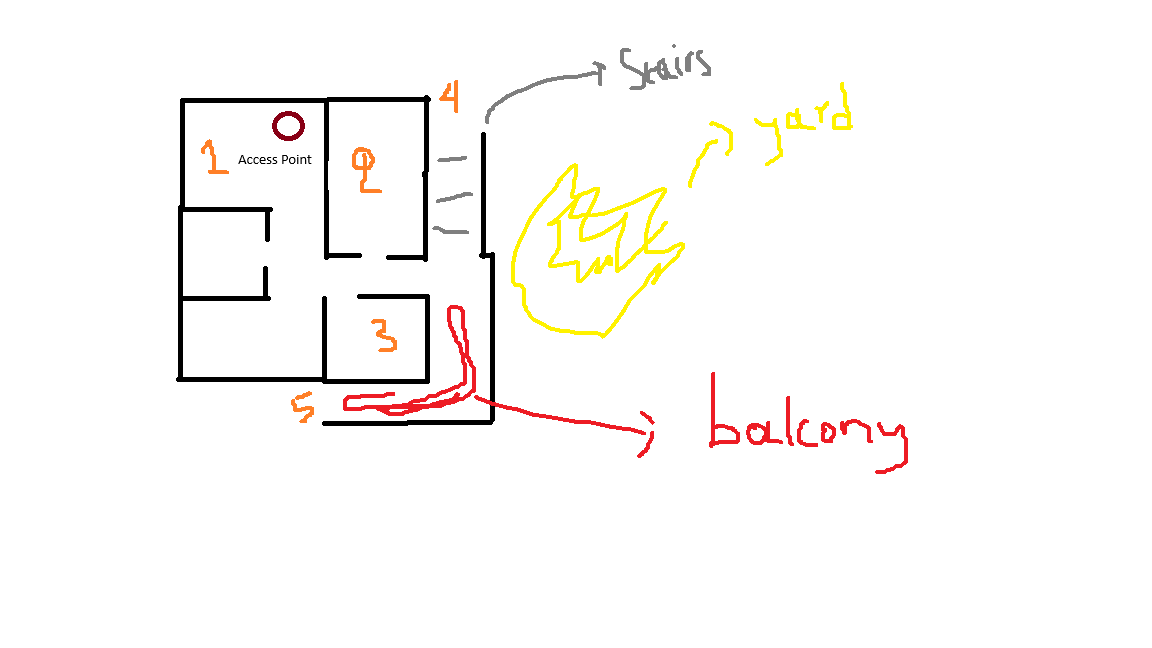
\includegraphics[width=1.5\textwidth]{images/topology.png}
    \caption{My topology and the measurement points for iperf. The sections that are written on the image are stairs, yard and balcony. Note that in front of the AP there are windows and a balcony.}
    \label{fig:topology}
\end{figure}

The devices that I am going to use are: 

\begin{itemize}
    \item Desktop: connected to the AP with an Ethernet cable. Speed: 1000Mb/s. IP: 192.168.1.135
    \item Laptop: connected to the AP with a wireless interface. Theoretical max speed of the wireless card Qualcomm Atheros QCA9377 at 5 GHz, Speed: 433Mbps. IP: 192.168.1.169
    \item Tablet: connected to the AP with a wireless interface and will have the WiFi analyzer app. Theoretical max speed of the wireless card Qualcomm WCN3980 at 5GHz: Speed: 433Mbps. IP:192.168.1.168.
    \item Access point: COSMOTE-178276
\end{itemize}
\section{Question 1}

\textbf{Regarding the following subquestions here is a brief overview:} 

The samples were collected using my tablet at measurement points 3 and 1. Note that since I live in a rural area there aren't many access points available. For that reason, to collect as many signals as possible, the 2.4GHz spectrum should be used. This also means that its not possible to find many APs above the -60dBm range or even the -70dBm to -60dBm. The ranges will be modified to: 

\begin{enumerate}
    \item Name: \textbf{C1}: $-50 \rightarrow -70$
    \item Name: \textbf{F1}: $-70 \rightarrow -80$ 
    \item Name: \textbf{F2}: $-80 \rightarrow \infty$
\end{enumerate}. 

Additionally since rural areas receive less frequent infrastructure updates, technology might be outdated. 

(a) Select two spots in your house: one relatively close to the Access Point (AP) and one farther away from the AP.
Using the mobile application WiFi Analyzer, record for both spots the number of wireless networks within the range of your mobile device that have a signal strength (dBm):

\begin{enumerate}
    \item Greater than -60 dBm,
    \item In the range between -70 dBm and -60 dBm, and
    \item Less than -70 dBm.
\end{enumerate}

Note that the signal strength may fluctuate over time.
For this reason, you can take the average value of several (e.g., 3–5) signal strength measurements.
Present your measurements in a table.


\subsection{Answer a}

Since there aren't many networks to sample the number of networks in each range can be seen below. These sometimes include the same networks for the close and far range. For example COSMOTE-178276 is counted for both C1 and F1.


\begin{center}
\begin{tabular}{| c | c |}
    \hline
     Range & Number  \\
     \hline
     C1 & 1 \\
     \hline
     F1 & 2 \\
     \hline
     F2 & 2\\
     \hline
\end{tabular} 
\end{center}


\begin{center}
\begin{tabular}{| c | c | c | c | c |}
    \hline
     Name & Spectrum & Distance To AP & Signal Strength & Mean\\
     \hline
     COSMOTE-178276 &  2.4GHz & Far & -77dBm, -76dBm, -73dBm, -74dBm & -75dBm\\
     \hline
     COSMOTE-178276 &  2.4GHz & Close & -57dBm, -52dBm, -49dBm, -42dBm & -50dBm \\
     \hline
     COSMOTE-190032 &  2.4GHz & Close & -94dBm, -95dBm & -94.5 dBm\\
     \hline
     COSMOTE-315796 & 2.4GHz & Far & -84dBm,-80dBm, -88dBm, -87dBm & -84.75dBm\\
     \hline
     COSMOTE-315796 & 2.4GHz & Close & not in range & not in range\\
     \hline
     COSMOTE-686079 & 2.4GHz & Far & -76dBm, -78dBm, -76dBm, -78dBm & -77dBm\\
     \hline
     COSMOTE-686079 &  2.4GHz & Close & not in range  & not in range \\
     \hline
\end{tabular} 
\end{center}

\pagebreak 
(b) For the wireless networks you recorded in the previous sub-question — specifically those with signal strength greater than -60 dBm and those with signal strength between -70 dBm and -60 dBm — assign each network a name such as A1, A2, and so on.
Also, record their transmission channel.

Present your measurements in a table, which should include the signal strength and the transmission channel of your own wireless network as well.

Based on the information from the table, which channel would you recommend for your own network and why?
How does your recommendation compare with the channel rating provided by the WiFi Analyzer application?
(The rating is usually available through the “rating” option/window in the app.)


\subsection{Answer b}
Since we don't have many samples for the above ranges we are going to use the ranges described in the brief: 

\begin{itemize}
    \item C1
    \item F1
    \item F2: using the COSMOTE-315796 network
\end{itemize}

The networks of these ranges are going to be named like this: 

\begin{itemize}
    \item  $\text{COSMOTE-178267} \rightarrow APClose$ for the close distance measurement of our own network's AP.
    \item $\text{COSMOTE-178267} \rightarrow APFar$ for the far distance measurement of our own network's AP.
    \item $\text{COSMOTE-686079} \rightarrow CosmoteFar_1$ for the far distance measurement of the remote AP.
    \item $\text{COSMOTE-315796} \rightarrow CosmoteFar_2$ for the far distance measurement of the remote AP.
\end{itemize}

\begin{center}
\begin{tabular}{| c | c | c | c | c | c |}
    \hline
     Name & Spectrum & Distance To AP & Signal Strength & Link Speed & Channel \\
     \hline
     APClose &  2.4GHz & Close & -50dBm & 150Mbps 40MHz& CH 9 (11) \\
     \hline
     APFar &  2.4GHz & Far & -75dBm &  45Mbps 40MHz& CH 9 (11)\\
     \hline
     $CosmoteFar_1$&  2.4GHz & Far & -77dBm & 40Mbps  40MHz & CH 6 (4)\\
     \hline
     $CosmoteFar_2$&  2.4GHz & Far & -84.75dBm & 20Mbps  40MHz & CH 9 (7)\\
     \hline
\end{tabular} 
\end{center}

\subsubsection{Channel rating in the far point} 
\begin{figure}[H]
    \centering
    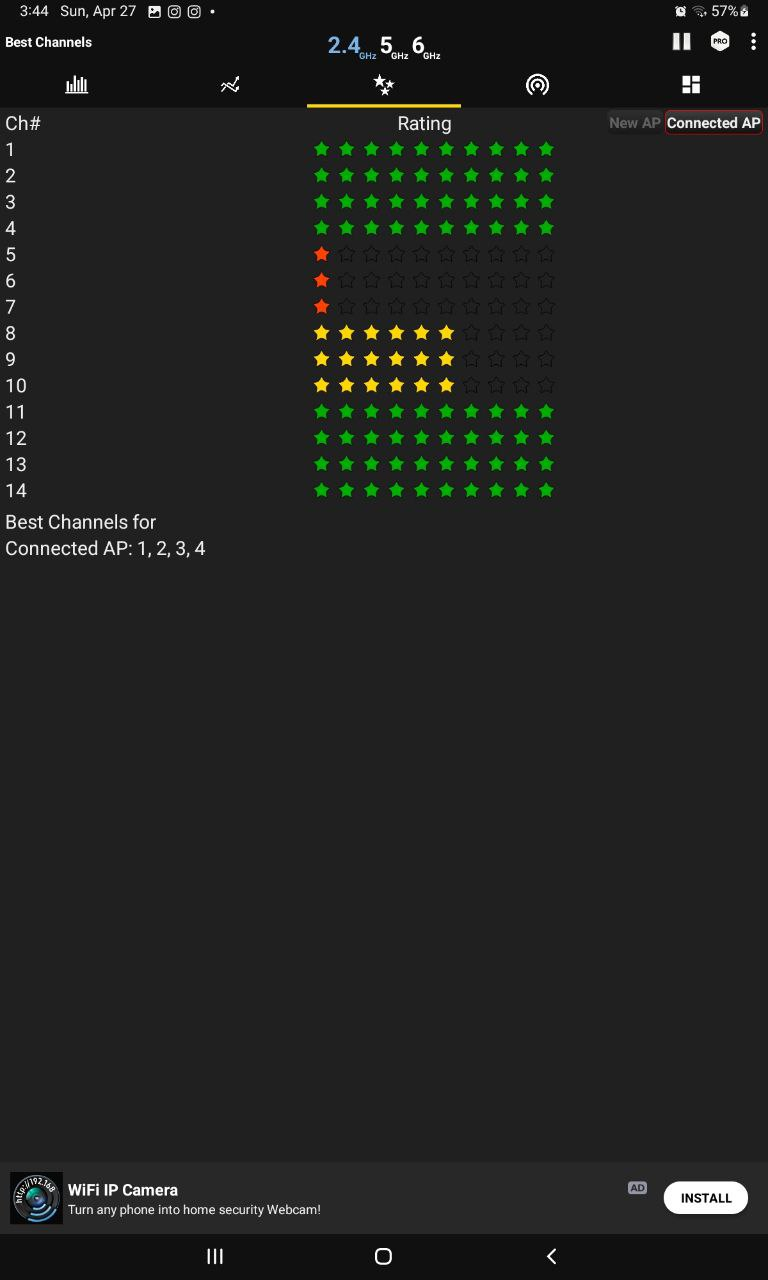
\includegraphics[width=1\linewidth]{images/rating_far.jpg}
    \caption{Rating assigned to channels by the app.}
    \label{fig:rating-far}
\end{figure}

\begin{figure}[H]
    \centering
    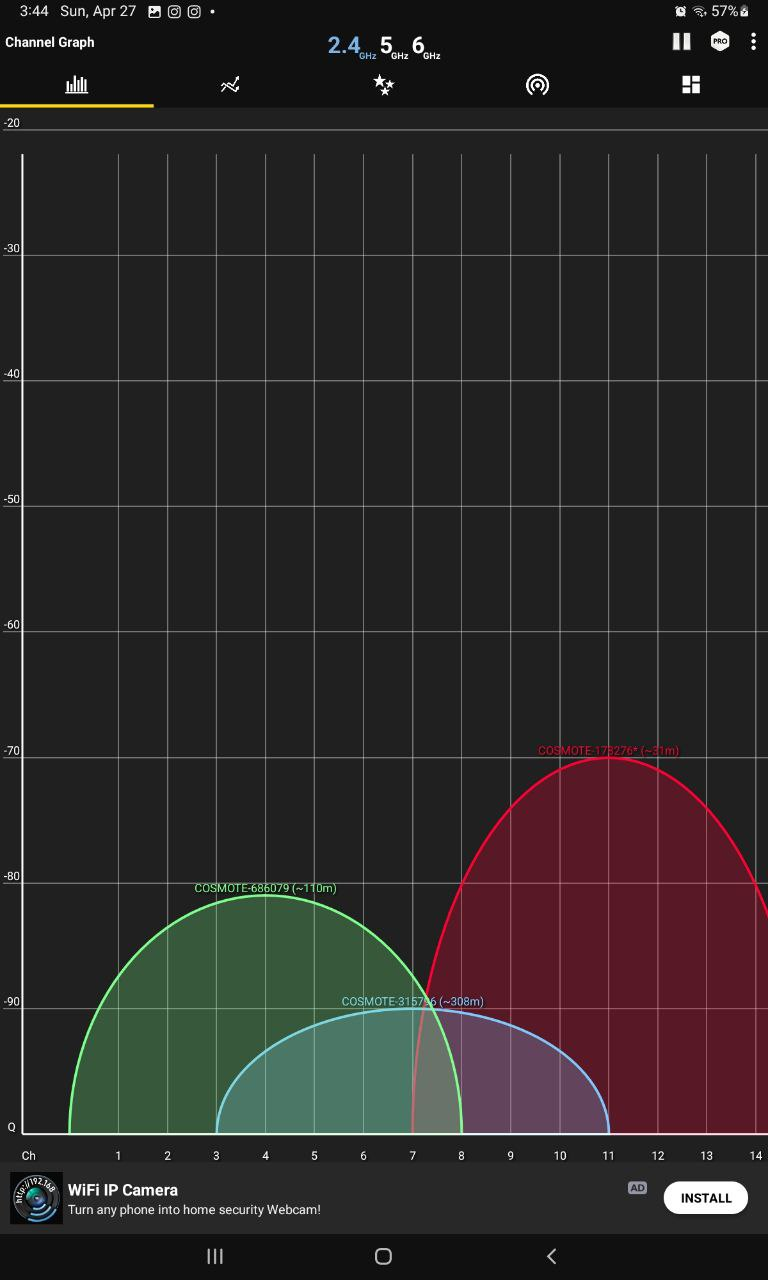
\includegraphics[width=1\linewidth]{images/channels_used_far.jpg}
    \caption{Channels used by the networks.}
    \label{fig:channels-used-far}
\end{figure}

\subsubsection{What channel should our network's AP use?}

I recommend using channels 11 to 13.
This range experiences minimal interference from neighboring networks, providing a cleaner spectrum and improving overall signal quality and stability. It also introduces less interference to neighboring networks from our own.

The application suggests using channels in the 1–3 and 11–14 ranges.
However, the 1–3 range should not be rated with five stars, as interference is clearly present.
This can be observed in Figure 3 \ref{fig:channels-used-far}, where the network $CosmoteFar_1$ overlaps with channels 1–3, causing potential interference.
In contrast, the 11–14 range is correctly assigned a five-star rating, as there are no overlapping networks observed in this range.
The remaining channels are appropriately rated with a lower score due to the high level of interference detected from neighboring networks.

\subsubsection{Channel rating in the close point}
\begin{figure}[H]
    \centering
    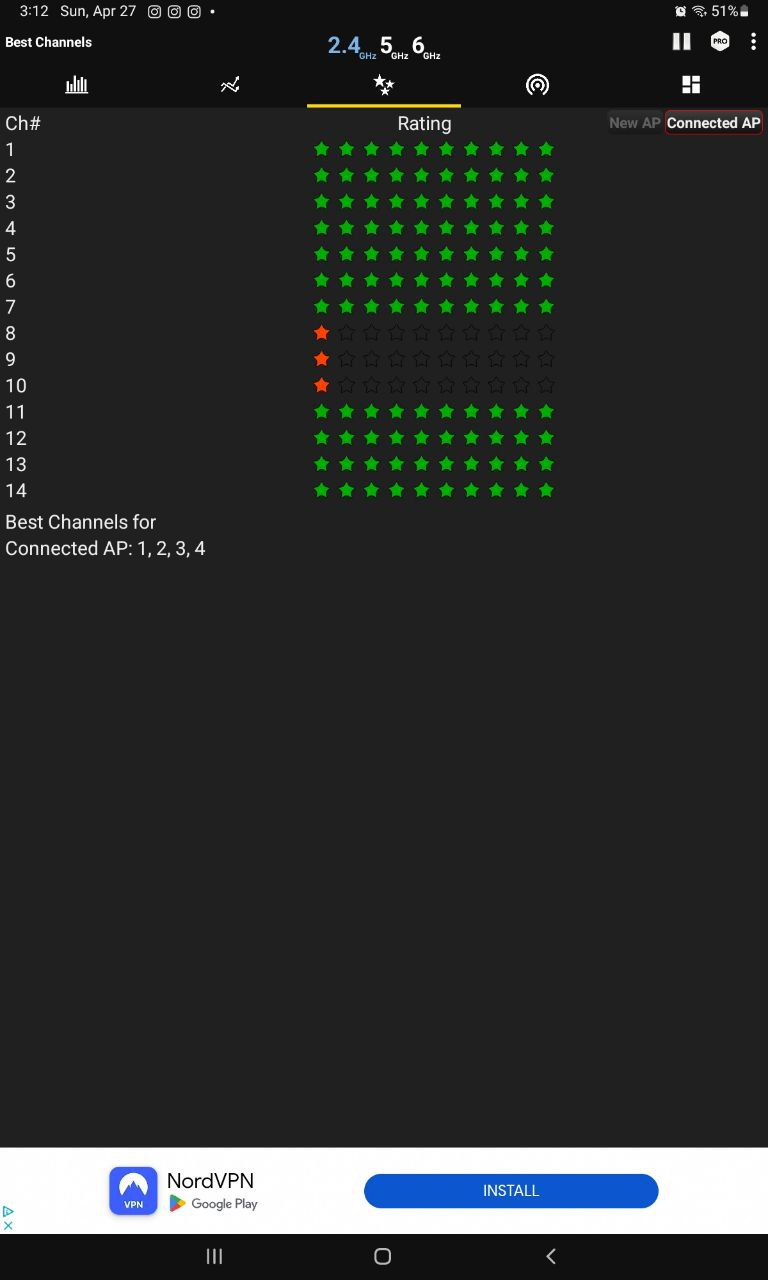
\includegraphics[width=1\linewidth]{images/rating_close.jpg}
    \caption{Rating assigned to channels by the app.}
    \label{fig:rating-close}
\end{figure}

\begin{figure}
    \centering
    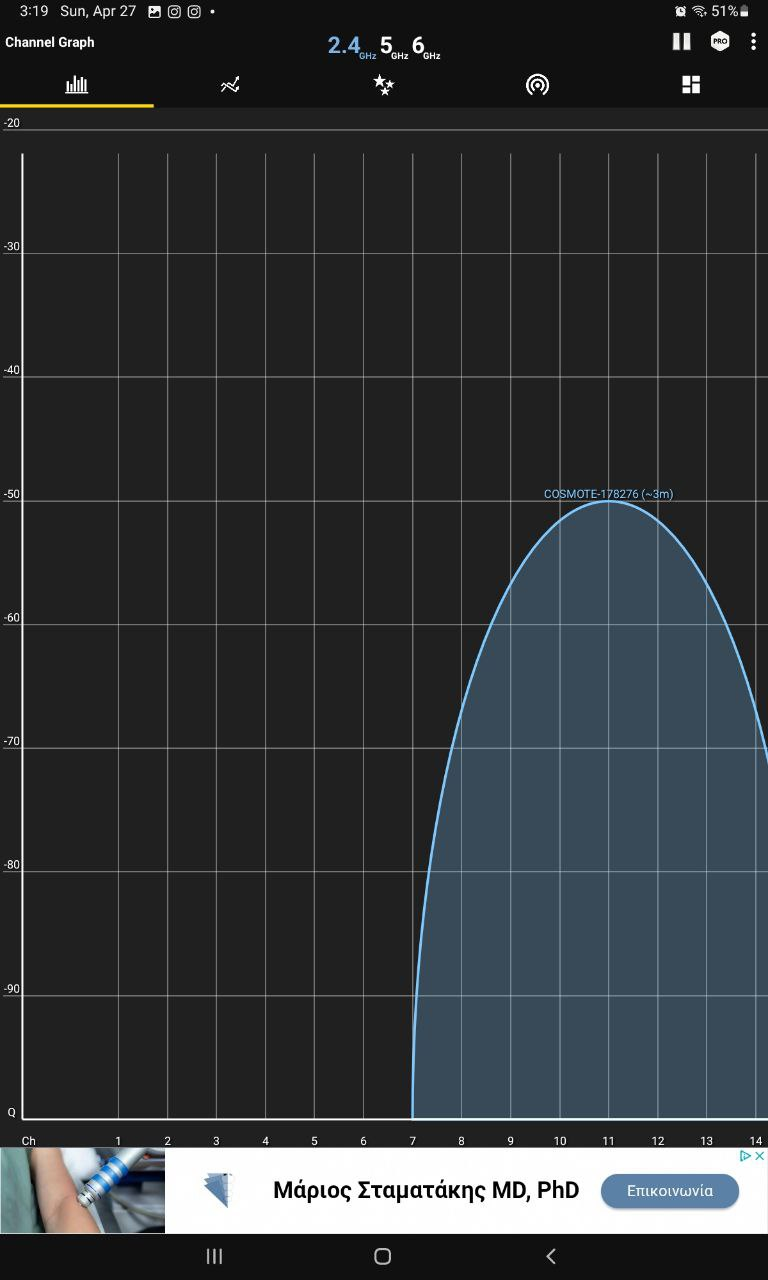
\includegraphics[width=1\linewidth]{images/channels_used_close.jpg}
    \caption{Channels used by the networks.}
    \label{fig:channels-used-close}
\end{figure}

\subsubsection{What channel should our network's AP use?}

In this case, there is minimal to no interference from neighboring networks.
The WiFi spectrum is relatively clean, and any channel between 1 and 14 could be used, with good expected performance.
According to the app's rating Figure \ref{fig:rating-close}, channels 8 to 10 are strongly discouraged for use, as they receive very low ratings.
The exact reason for this is unclear, especially since the channel graph Figure \ref{fig:channels-used-close} shows no significant network activity in that range.
It is possible that background interference or hidden networks (not detected during the scan) influenced the app’s evaluation.

\section{Question 2}
For the TCP throughput measurements, you will need to run the iperf3 application on your laptop/desktop with the -s option (server mode).

Select five points in your house at different distances from the AP (Access Point) of your wireless network.
The selected points should include:

\begin{enumerate}
    \item one very close to the AP,
    \item one far from the AP,
    \item and the remaining three at intermediate distances.
\end{enumerate}

At each of the selected points, place your mobile device and measure:

\begin{enumerate}
    \item the signal strength from your AP,
    \item the Wi-Fi interface speed (link speed or transmission rate),
    \item the TCP throughput.
\end{enumerate}

The signal strength can be measured using the WiFi Analyzer application.
The Wi-Fi interface speed (link speed) can be found by displaying the interface information (on mobile) or checking the interface status (on Windows/Linux).

Finally, the TCP throughput can be measured by running the iperf3 application on the mobile device (or a second laptop) with the -c option (client mode), providing the IP address of the laptop/desktop where the iperf server is running, along with the server's port number.

For the throughput measurement, take the average value of at least 5 measurements, with each measurement lasting 10 seconds.

Record the following in a table for each point:

the distance of the point from the AP,

the three measurements (signal strength, Wi-Fi interface speed, and average throughput).

Create two graphs:

The first graph should plot signal strength and Wi-Fi interface speed (on the same graph) as a function of distance from the AP.

The second graph should plot Wi-Fi interface speed and average throughput as a function of signal strength.

Answer the following questions:

i) What is the shape of the two graphs? Did you expect this shape?

ii) How would the first graph (A) change if the representation was a function of the logarithm of distance?

iii) In the second graph (B), how does the throughput compare with the Wi-Fi interface speed?
Did you expect this relationship?

\subsection{Answer}

The iperf3 server was run on my desktop with the Ethernet connection. The throughput measurements were carried out using a laptop and iperf3. It was set up to run the following command: 
\begin{lstlisting}
iperf3 -c <hostname> -t 60 -i 10 > iperf3_output.txt
\end{lstlisting}

5 measurements of the above configuration were carried at each spot. In order to obtain the signal strength and the link speed the following command was used: 

\begin{lstlisting}
$ iw dev wlp4s0 link
Connected to 74:06:35:89:ba:84 (on wlp4s0)
	SSID: COSMOTE-178276
	freq: 5500.0
	RX: 16697197 bytes (190107 packets)
	TX: 888979574 bytes (579832 packets)
	signal: -75 dBm
	rx bitrate: 130.0 MBit/s VHT-MCS 3 80MHz short GI VHT-NSS 1
	bss flags: short-slot-time
	dtim period: 1
	beacon int: 100  
\end{lstlisting}

The following is the table containing the measurements: 

\begin{tabular}{| c | c | c | c |}
    \hline
     Distance To AP & Signal Strength & Link Speed & Throughput (Mbps)\\
     \hline
     Very Close (1) & -40dBm & 433-390Mbps & 300.00,275.33,269.83,301.50,300.83=289.498  \\
     \hline
     Intermediate (2) & -58dBm & 390-195.5Mbps & 263.83,255.67,256.50,249.17,218.50=248.734  \\
     \hline
     Intermediate (3) & -74dBm & 195-130Mbps & 107.34,107.39,51.31,77.76,107.64=90.288 \\
     \hline
     Intermediate (4) & -62dBm & 72.2-7.2Mbps & 42.75,40.59,40.94,42.15,40.54=41.394 \\
     \hline
     Far (5) & -86dBm & 14.4-5.5Mps & 11.93,10.38,11.43,10.08,10.57=10.878 \\
     \hline
\end{tabular} 

\subsubsection{Graphs}
\begin{figure}[H]
    \centering
    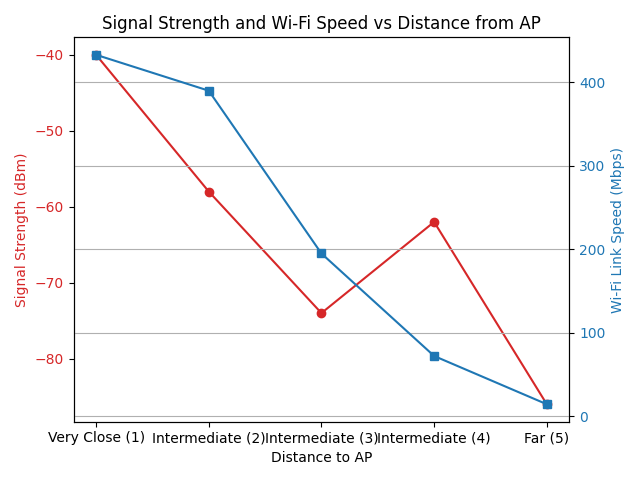
\includegraphics[width=1\linewidth]{images/signal_strength_wifi_speed_distance.png}
    \caption{Signal strength and Wi-Fi link speed as a function of distance from the Access Point. As distance increases, signal strength decreases and link speed generally drops.}
    \label{fig:signal-strength-wifi-speed-distance}
\end{figure}

\begin{figure}[H]
    \centering
    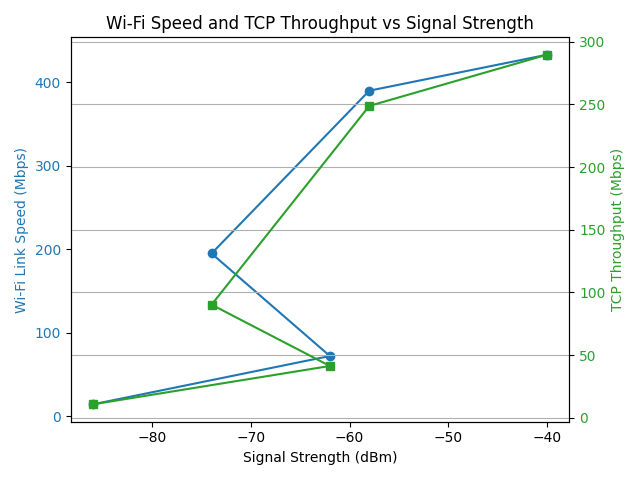
\includegraphics[width=1\linewidth]{images/wifi-speed-throughput-signal-strength.png}
    \caption{Wi-Fi link speed and TCP throughput as functions of signal strength. Both metrics generally improve as the signal becomes stronger (closer to 0 dBm).}
    \label{fig:signal-strength-wifi-speed-distance}
\end{figure}
\subsubsection{i) What is the shape of the two graphs? Did you expect this shape?}
\begin{itemize}
    \item Graph A (Signal Strength \& Link Speed vs. Distance): Both curves fall off as distance increases—signal strength drops (more negative dBm) and link speed declines. It’s essentially a monotonically decreasing trend (with a small local “bump” at point 4), resembling the classic path-loss decay you’d expect as you move away from an AP. Perhaps the bump is due to better multipath signals.
    \item Graph B (Link Speed \& Throughput vs. Signal): Both link speed and TCP throughput rise together as signal improves (moves from –85 dBm toward –40 dBm). The two metrics track each other closely in a roughly linear, positive-correlation fashion.
\end{itemize}


Yes—these shapes are exactly what one predicts: Wi-Fi suffers increasing path loss (hence lower link rates) with distance, and higher signal levels yield higher link rates and real-world throughput.
\subsubsection{ii) How would the first graph (A) change if the representation was a function of the logarithm of distance?}
If you re-plot signal and speed versus log(distance) instead of linear “distance category,” the curves would straighten out into something closer to a linear decline. In wireless path-loss theory, power falls off proportional to $\frac{1}{d^n}$, so on a log-distance scale you see an approximately straight line rather than a steep curve.
\subsubsection{iii) In the second graph (B), how does the throughput compare with the Wi-Fi interface speed? Did you expect this relationship?}
Throughput (green) consistently runs below the raw link speed (blue), but follows the same upward trend. That is, at –60 dBm your device might link at ~400 Mbps but achieve ~260 Mbps TCP. This gap is expected—overheads (MAC/PHY framing, retransmits, protocol inefficiencies) mean real TCP rates are typically a portion of the negotiated link rate.
\end{document}

